%
% File emnlp2020.tex
%
%% Based on the style files for ACL 2020, which were
%% Based on the style files for ACL 2018, NAACL 2018/19, which were
%% Based on the style files for ACL-2015, with some improvements
%%  taken from the NAACL-2016 style
%% Based on the style files for ACL-2014, which were, in turn,
%% based on ACL-2013, ACL-2012, ACL-2011, ACL-2010, ACL-IJCNLP-2009,
%% EACL-2009, IJCNLP-2008...
%% Based on the style files for EACL 2006 by 
%%e.agirre@ehu.es or Sergi.Balari@uab.es
%% and that of ACL 08 by Joakim Nivre and Noah Smith

\documentclass[11pt,a4paper]{article}
\usepackage[hyperref]{emnlp2020}
\usepackage{times}
\usepackage{latexsym}
\renewcommand{\UrlFont}{\ttfamily\small}

\usepackage{graphicx}
\usepackage{xcolor}
\usepackage{longtable}
\usepackage{tikz}
\usetikzlibrary{calc}
\usepackage[draft]{todo}
\usepackage{xspace}
\usepackage{amsmath,amsfonts,amssymb}
\usepackage{mathrsfs}
\newcommand{\R}{\ensuremath{\mathbb{R}}}

% This is not strictly necessary, and may be commented out,
% but it will improve the layout of the manuscript,
% and will typically save some space.Boldface denotes significant gains with respect to \system{Mix-Nat} (or \system{Mix-Nat-RNN}, for WDCMT), underline denotes significant losses.
\usepackage{microtype}

%\aclfinalcopy % Uncomment this line for the final submission
%\def\aclpaperid{***} %  Enter the acl Paper ID here

%\setlength\titlebox{5cm}
% You can expand the titlebox if you need extra space
% to show all the authors. Please do not make the titlebox
% smaller than 5cm (the original size); we will check this
% in the camera-ready version and ask you to change it back.

\newcommand{\fyTodo}[1]{\Todo[FY:]{\textcolor{orange}{#1}}}
\newcommand{\fyTodostar}[1]{\Todo*[FY:]{\textcolor{orange}{#1}}}
\newcommand{\fyDone}[1]{\done[FY]\Todo[FY:]{\textcolor{orange}{#1}}}
\newcommand{\fyFuture}[1]{\done[FY]\Todo[FY:]{\textcolor{red}{#1}}}
\newcommand{\fyDonestar}[1]{\done[FY]\Todo[FY:]{\textcolor{orange}{#1}}}
\newcommand{\jcTodo}[1]{\Todo[JC:]{\textcolor{red}{#1}}}
\newcommand{\jcDone}[1]{\done[JC]\Todo[JC:]{\textcolor{red}{#1}}}

\newcommand{\mpTodo}[1]{\Todo[MP:]{\textcolor{green}{#1}}}
\newcommand{\mpDone}[1]{\done[MP]\Todo[MP:]{\textcolor{green}{#1}}}
\usepackage{mathtools,xparse}
\DeclarePairedDelimiter{\abs}{\lvert}{\rvert}
\DeclarePairedDelimiter{\norm}{\lVert}{\rVert}
\NewDocumentCommand{\normL}{ s O{} m }{%
  \IfBooleanTF{#1}{\norm*{#3}}{\norm[#2]{#3}}_{2}%
}
\newcommand{\src}{\ensuremath{\mathbf{f}}} % source sentence
\newcommand{\trg}{\ensuremath{\mathbf{e}}} % target sentence
\newcommand{\domain}[1]{\texttt{\textsc{#1}}}
\newcommand{\system}[1]{\texttt{\textbf{#1}}}
\newcommand{\vlambda}{\ensuremath{\boldsymbol\lambda}\xspace} % parameters vector for a distribution
\newcommand{\indic}[1]{\ensuremath{\mathbb{I}(#1)}}
% \newcommand{\SB}[1]{\textcolor{green}{#1}}
% \newcommand{\SW}[1]{\textcolor{red}{#1}}
\newcommand{\SB}[1]{\textbf{#1}}
\newcommand{\SW}[1]{\underline{#1}}
\renewcommand\textfraction{.1}
\renewcommand\floatpagefraction{.95}

\newcommand\BibTeX{B\textsc{ib}\TeX}

\iffalse   % removes draft highlighting for final version
\renewcommand{\draftAdd}[2]{#1}
\fi

% -- \title{Ablation study on the residual adapter in Neural Machine Translation}
\title{A Study of Residual Adapters for Multi-Domain Neural Machine Translation}

\author{First Author \\
  Affiliation / Address line 1 \\
  Affiliation / Address line 2 \\
  Affiliation / Address line 3 \\
  \texttt{email@domain} \\\And
  Second Author \\
  Affiliation / Address line 1 \\
  Affiliation / Address line 2 \\
  Affiliation / Address line 3 \\
  \texttt{email@domain} \\}

\date{}

\begin{document}
\maketitle
\begin{abstract}
% Among the approaches for adapting a pretrained NMT model to a specific domain, finetuning is the dominant method. Finetuning proposes 2 approaches: simply continuing training all the parameters \cite{Luong15stanford}; training addition adapters while freezing the pretrained model\cite{Bapna19simple,Vilar18learning}. The second approach has several advantages including preserving the pretrained model and the legerity of the adapters. However, the behavior of these adapters has not been further studied. The objective of this paper is to give an ablation study on the use of residual adapter in the domain adaptation problem.
% \mpTodo{correcting abstract}
% **** 
\fyDone{Citation-free abstract}
Domain adaptation is an old and vexing problem for machine translation systems. The most common approach and successful to supervised adaptation is to fine-tune a baseline system with in-domain parallel data. Standard fine-tuning however modifies all the network parameters, which makes this approach computationally costly and prone to overfitting. A recent, lightweigth approach, instead augments a baseline model with supplementary (small) adapter layers, keeping the rest of the mode unchanged. This has the additional merit to leave the baseline model intact, and adaptable to multiple domains. In this paper, we conduct a thorough analysis of the adapter model in the context of a multidomain machine translation task. We contrast multiple implementations of this idea on two language pairs. Our main conclusions is ..\fyTodo{abstract to be continued}

\end{abstract}
\section{Introduction } \label{sec:intro}
\mpTodo{write introduction} \fyDone{Citations in chronological order}\fyDone{Split long sentences}
Owing to multiple improvements, Neural Machine Translation(NMT) \cite{Kalchbrenner13recurrent,Sutskever14sequence,Bahdanau15learning,Vaswani17attention} nowadays delivers useful outputs for many language pairs. However, as many deep learning model, NMT models need to be trained with sufficiently large amounts of data to reach their best performance. Therefore, the quality of translation of NMT model is still limited in low-resource language and low-resourced domain conditions \cite{duh13adaptation,zoph16transfer,koehn17six}. While many approaches have been proposed to improve the quality of NMT models in low-resource domains (see the recent survey of \citet{Chu18asurvey}), full fine-tuning of a generic baseline model remains the dominant supervised approach when adapting NMT models to specific domains \cite{Luong15stanford,neubig18rapid}.

Under this view, building adapted systems is a two-step process: (a) one first trains NMT with the largest possible parallel corpora, possibility aggregating texts from multiple, heterogeneous sources; (b) assuming that in-domain parallel documents are available for the domain of interest, one then adapts the pre-trained model by resuming training with the sole in-domain corpus. It is a conjecture that pre-trained model constitute a better initialization than a random one, especially when the adaptation data is scarce. Indeed, studies of transfer learning for NMT such as \cite{artetxe20cross,aji20neural} have confirmed this claim by extensive experiments. Full fine-tuning, that adapts all the parameters of a baseline model usually significantly improves the quality of the NMT for the chosen domain. However, it also yields large losses in translation quality for other domains, a phenomenon referred to as ``catastrophic forgetting'' in the neural network literature \cite{McCloskey89catastrophic}. Therefore, a fully fine-tuned model is only useful to one target domain. As the number of domains to handle grows, training and maintaining a separate model for each task can quickly becomes tedious and resource-expensive .\fyDone{Fix this sentence.}

\cite{Vilar18learning,Bapna19simple} have recently proposed a simple and lightweight domain adaptation method that also preserves the value of pre-trained models, based on small adapters component that are plugged in each hidden layer. These adapters are trained only with the in-domain data, keeping the pre-trained model frozen. Because these additional adapters are very small compared to the size of the baseline model, their use significantly reduces the cost of training and maintaining fine-tuned models, while still delivering a performance that is close to that of full fine-tuning.

In this paper, we would like to extend this architecture to improve NMT in several settings that still challenge automatic translation, such as translating texts from multiple topics, genre or domains, in the face of unbalanced data distribution. Furthermore, as the notion of ``domains''  is not always well established, another practical setting is the translation of texts mixing several topics / domains. Finally, another requirement is the need to also translate texts from domain unseen in training, based only on the unadapted system, which should be made as strong as possible. 
% Residual adapters allow us to adapt NMT model to any specific domain in a computationally cheap way. Could we adapt NMT model to noisy text and topical text at once? While residual adapters are good at adapting to one specific domain, their performance still dramatically decrease for the other domains seen in training, as we show in our experiments. Therefore, we have to decide whether to use residual adapters manually, i.e, we have to know to which domain the text belongs a priori. Therefore, we would like to fuse a domain classifier to the architecture in order to weight the contribution of the adapters with respect to the topic-relatedness of the text.
\fyDone{Say differently: various implementations}

In this context, our main contribution is a thorough experimental study of the use of residual adapters in multi-domain translation. We notably explore ways to adjust and/or regularize adapter modules to handle situations where the adaptation data is very small. We also propose and contrast two new variants of the residual architecture: in the first one (highway residual adapters), adaptation still affects each layer of the architecture, but its effect is delayed till the last layer, thus making the architecture more modular and adaptive; in the second one (gated residual adapters), we explore ways to improve the performance in the face of train-test data mismatch. We experiment with two language pairs and report results that demonstrate the flexibility and effectiveness of these architectures. 
\fyDone{One bit of a conclusion here}\fyFuture{Build a proper training scenario for these two conditions}

\section{Residual adapters \label{sec:res}}

\subsection{Basic architecture \label{ssec:architecture}}
\fyDone{More contexts and notations from the transformer}\fyDone{Encoder / decoder layers}

\subsubsection{The computation of adapter layers}
Our reference architecture is the Transformer model of \cite{Vaswani17attention}, which we assume contains a stack of layers both in the encoder and the decoder side. Each layer contains two subparts, an attention layer and a dense layer. Details may vary from one implementation to another, we simply content here that each layer $i \in \{1 \dots L\}$ (in the encoder or the decoder) computes a transform of a fixed-length sequence of $d$-dimensional input vectors $h^{i-1}$ into a sequence of output vectors $h^{i}$.

The residual adapter architecture extends this model by adding one new computational module for each layer. The $i^{\text{th}}$ such residual adapter thus modifies $h^i$ by computing the following transformations:\fyDone{Use align env}
\begin{align*}
  h^{i}_1 &= \mathbf{W}_{db}^{i}h^{i} + b^i_{1} \\
  h^{i}_2 &= \mathbf{ReLU}(h_1^{i}) \\
  h^{i}_3 &= \mathbf{W}_{bd}^{i}h_2^{i} + b^i_{2} \\
  \bar{h}^{i} &= h^{i}_3 + h^i.
\end{align*}
Overall, the  $i^{\text{th}}$ adapter is thus parameterized by matrices $\displaystyle{\mathbf{W}_{db}^{i}\in\mathbb{R}^{d\times b}}$,$\displaystyle{\mathbf{W}_{bd}^{i}\in\mathbb{R}^{b\times d}}$, bias vectors $\displaystyle{b^i_{1} \in \mathbb{R}^{b}}$, $\displaystyle{b^i_{2} \in \mathbb{R}^{d}}$, with $b$ the dimension of the adapter (with $d \gg b$)\fyTodo{Check this}. For the sake of brevity, we will simply denote $h^{i}_3 = \operatorname{ADAP}^{(i)}(h^i)$, and $\theta_{\operatorname{ADAP}^{(i)}}$ the corresponding set of parameters.\fyDone{or is it $h_i$ ?}\fyDone{attention aux matrices $W_i$}

The "adapted" hidden vectors $\bar{h}^i_{ 1\leq i \leq L-1}$, where $L$ is the number of layers, will then be the input of the $(i+1)^{\text{th}}$\fyDone{Self attention ?} layer; $\bar{h}^L$ is passed to the decoder if it belongs to the encoder side, or is the input of output layer if it belongs to the decoder side. Note that zeroing out all adapters enables us to recover the basic Transformer, with $\bar{h}^{i} = h^i$ for all $i$.

In the experiments reported in Section~\ref{sec:exp}, we will use $2\times{}L=12$ residual adapters, one for each of the $L=6$ attention layers of the encoder and similarly for the decoder.\footnote{In the decoder, the stack of self-attention layers and cross encoder-decoder attention only counts as one attention layer and only serves one residual adapter.}

\subsubsection{Design space and variants}
This general architecture leaves open many design choices pertaining to the details of the network organization, the training procedure and the corresponding objective function.

A first question concerns the number of adapter layers. While in principle, all Transformer layers can be subject to adaptation, it is nonetheless worthwhile to consider simpler adaptation schemes, which would only alter a limited number of layers. Such strategy might be especially relevant when the training corpus contains very small domains, such as the ones considered in our experiments, and for which a complete adaptation may not be necessary or/and or prone to overfitting. Likewise, it might be meaningful to explore ways to share subsets of adapters across domains. This in turn raises the issues of which layer(s) to adapt, a question that can be approached in the light of recent analyses of the Transformer architecture which conjectured that the higher layers encode more global patterns with a more ``semantic'' interpretation, while the lower layers encode more local patterns akin to morpho-syntactic information \cite{raganato18analysis}.

% The size of available corpora for each domain is extremely varying. For example, the corpus of domain \domain{tourism} in En-De contains only around $7\times10^3$ sentence pairs while the corpus of domain \domain{news} in En-De contains approximately $3\times10^6$ sentence pairs. For extremely small domains, we could economize the number of parameters by reducing the number of residual adapters in the architecture. While only a limited number of adapters are incorporated to the NMT model, which positions in the model are more important in the domain adaptation task? We would like to analyze the impact of position and number of residual adapters involved in the adapted model. It is conjectured that the higher layers represent more global patterns such as semantic while the lower layers represent more local patterns such as syntactic \cite{raganato18analysis}\fyTodo{Missing reference here}. The domain shift in local patterns and global patterns has not yet studied. In this paper, we do not intend to study this aspect of the domain adaptation problem. We would like to give an extensive comparison between domain adaptation in different levels in NMT model. 

A related question concerns the regularization of adapter layers to mitigate overfitting. Reducing the number of adapters, or their dimensions, is simple, but these choices are difficult to optimize numerically -- an issue that becomes important as the number of domain grows. Less naïve alternatives can also be entertained, such as applying weight decay or layer regularization to the adapter. Implementing these requires to modify the objective function in a way that still allows for a smooth optimization problem. For instance, weight decay applies a penalization on the weights of the adapters, complementing the cross-entropy term with a function of the norm of the parameters: \fyDone{The second summation also runs over $x,y$ ? I think not}
\begin{equation*}
  \begin{split}
    \bar{L} & = \frac{1}{\#(x,y)}\mathop{\sum}_{x,y}( - \log(P(y|x))) \\
    & + \lambda  \sum_{i \in \{1,..,6\} \otimes \{enc, dec\}} \normL{\theta_{\operatorname{ADAP}^{(i)}}}
  \end{split}
\end{equation*}
An alternative scheme is \emph{layer regularization}, which penalizes the output of the adapters, corresponding to the following new training objective:
\begin{equation*}
  \begin{split}
    \bar{L} & = \frac{1}{\#(x,y)}\mathop{\sum}_{x,y} (-\log(P(y|x)) \\
    & + \lambda \sum_{i \in \{1,..,6\} \otimes \{enc, dec\}} \normL{\operatorname{ADAP}^{(i)}(h_i(x,y))})
  \end{split}
\end{equation*}

Finally, another independant design choice relates to the training strategy for adapters. A first option is to generalize supervised domain adaptation to multi-domain adaptation and to proceed in two steps: (a) train a generic model with all the available data; (b) train eacj adapter layer with domain-specific data, keeping the generic model parameters unchanged. Another strategy is to adopt the view of \citet{Dredze08online}, where the multi-domain setting is viewed as an instance of multi-task learning \cite{Caruana97multitask}, where each domain corresponds to a specific task. This suggest to train the models as it were in a multi-task mode, training all the parameters from scratch: the generic parameters values will still depend on all the available data, while each adapter will only be trained with the corresponding in-domain data.

\subsection{Highway Residual Adapters \label{ssec:highway}}

In the basic architecture described in Section~\ref{ssec:architecture}, the computation performed by lower level layers will impact all the subsequent layers. In this section, we introduce an alternative implementation of the same idea, which however delays the adaptation of each layer to the last layer (of the encoder or the decoder) as represented on Figure~\ref{fig:hrl-architecture}. While the basic architecture performs adaptation in sequence, we propose here to perform it in parallel. This means that in this version, only the last hidden vector of the encoder (decoder) is modified according to:
\begin{equation}
  \bar{h}^L = h^L + \displaystyle{\mathop{\sum}_{1 \leq i \leq L} ADAP^i(h^i)} \label{eq:highway-output}
\end{equation}

One obvious benefit of this variant is that it allows us to reuse the hidden vectors $h^i$ of all hidden layers when computing an adapted output for several domains during the inference. In this situation, the forward step needs only to compute the hidden vectors $h^i$ once for the inner encoder layers, before an adapted sequence of vectors is computed at the topmost layer. Therefore, we can finetune the model to multiple domains at once without recomputing $h^i$. This variant also opens the way to more parameter sharing across adapters, a perspective that we will not explore further in this work. Instead, we use it to develop a second variation of the adapter model, that is presented in the next section.

\begin{figure}[htbp]
  \centering
  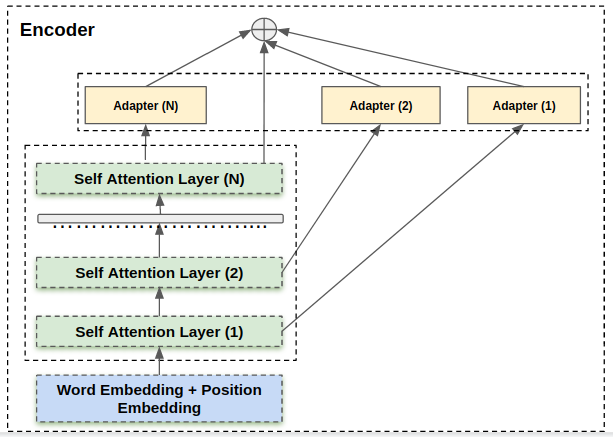
\includegraphics[scale=0.3]{fig/highway_residual}
  \caption{Highway multi-domain network with residual layers}
  \label{fig:hrl-architecture}
\end{figure}

\subsection{Gated Residual Adapters \label{ssec:gate}}
\mpTodo{Formalizing problem, network design, training algorithm}
The basic architecture presented above rests on a rather simplistic view of ``domains'' as made of well-separated and unrelated pieces of texts that are processed independently during the adaptation step. Likewise, when translating test documents, we need to make a choice between either using a specific domain-adapted model or resorting to the generic, unadapted model. In this context, errors on the domain label can have a strong (negative) impact on the trained model, or on the translation performance. 

Therefore, we would like to design a version of applying residual adapter that is more robust to such domains error. This variant, called the \emph{gated residual adapter models}, relies on the training of a supplementary trained component that will help decide whether to activate, on a word per word basis, a given residual layer, and to regulate the strength of this activation. To this end , we extend the highway version of residual adapters as follows.
\fyDone{Consistency of notations wrt section 2.1}

Formally, we replace the adapter computation of equation~\eqref{eq:highway-output} and take the adapted hidden (topmost) layer to be computed as (this is for domain $k$):
\begin{equation}
  \bar{h}^L = h^L + \displaystyle{\mathop{\sum}_{1 \leq i \leq L} \operatorname{ADAP}_k^i(h^i) \odot{} z_k(h^L)}, \label{eq:gated-output}
\end{equation}
where $z_k(h^L[t]) \in [0,1]$ measures the relatedness of the $t^{\text{th}}$ word $w_t$ to domain $k$. The more likely $w_t$ is in domain $k$, the larger $z_k(h^L[t])$ should be; conversely, for words\footnote{The term ``words'' here is employed by mere convenience as the system only manipulates sub-lexical BPE units; furthermore, the values of the hidden representations $h^{i}$ at position $t$ depends from all the other positions in the sentence.} that are not typical of any domain $k$ (eg.\ function words),  adaptation is minimum and the adapted corresponding encoder output ($\bar{h}^L[t]$) will remain close to the output of the generic model ($h^L[t]$). In our implementation, we incorporate two domain classifiers on top of the encoder and the decoder, that take the last hidden layer of the encoder (resp.\ decoder) as input and use the posterior probability $P(d=k|h^L[t]); \theta)$, with $\theta$ the set of all parameters, as the value of $z_k(h^L[t])$.

The training of gated residual adapters thus comprises three main steps, instead of two for the baseline version:
\begin{enumerate}
\item learn a generic model with mixed corpora comprising data from multiple domains.
\item train a domain classifier on top of the encoder and decoder; during this step, the parameters of the generic model are frozen. This model computes the posterior domain probability $P(k|h^L[t]; \theta)$ for each word $w_t$, based on the representation computed by the last layer.
\item train the parameters of adapters with in-domain data separately for each domain, while freezing the generic model and the domain classifiers.
\end{enumerate}
\fyFuture{is this classifier important, can we train with the rest of the system ?}

\section{Experimental settings \label{sec:exp}}

\subsection{Data and metrics \label{ssec:corpora}}
We perform our experiments with two translation pairs involving multiple domains: English-French (En$\rightarrow$Fr and English-German (En$\rightarrow$De). For the former pair, we use texts initially from 6~domains, corresponding to the following data sources: the UFAL Medical corpus V1.0 (\domain{med})\footnote{\url{https://ufal.mff.cuni.cz/ufal_medical_corpus}}, the European Central Bank corpus (\domain{bank}) \cite{Tiedemann12parallel}; The JRC-Acquis Communautaire corpus (\domain{law}) \cite{Steinberger06acquis}, documentations for KDE, Ubuntu, GNOME and PHP from Opus collection \cite{Tiedemann09news}, collectively merged in a \domain{it}-domain, Ted Talks (\domain{talk}) \cite{Cettolo12wit}, and the Koran (\domain{rel}). Complementary experiments also use v12 of the News Commentary corpus (\domain{news}). Corpus statistics are in Table~\ref{tab:Corpora-en-fr}.  Most corpora are available from the Opus web site.\footnote{\url{http://opus.nlpl.eu}}

\begin{table*}[htbp]
  \centering
  \begin{tabular}{ |lllllll|} %*{4}{|r|}}
    \hline
    %\multicolumn{4}{|l|}{Vocab size - En: 30,165, Fr: 30,398}\\
    \domain{med} & \domain{law} & \domain{bank} & \domain{it} & \domain{talk} & \domain{rel} & \domain{news} \\
    \hline
    2609 (0.68) & 190 (0.05)  & 501 (0.13) & 270 (0.07) & 160 (0.04) & 130 (0.03) & 260 (0) \\
    \hline
  \end{tabular}
\caption{Corpora statistics for En$\rightarrow$Fr : number of parallel lines ($\times 10^3$) and proportion in the basic domain mixture (which does not include the \domain{news} domain). \domain{med} is the largest domain, containing almost 70\% of the sentences, while \domain{rel} is the smallest, with only 3\% of the data.}
\label{tab:Corpora-en-fr}
\end{table*}

For En$\rightarrow$De, we use corpora distributed for the News task of WMT20\footnote{\url{http://www.statmt.org/wmt20/news.html}} including: European Central Bank corpus (\domain{bank}),  European Economic and Social Committee corpus (\domain{eco}), European Medicines Agency corpus (\domain{med})\footnote{\url{https://tilde-model.s3-eu-west-1.amazonaws.com/Tilde_MODEL_Corpus.html}}, Press Release Database of European Commission corpus, News Commentary v15 corpus, Common Crawl corpus (\domain{news}), Europarl v10 (\domain{gouv}) Tilde MODEL - czechtourism (\domain{tourism})\footnote{\url{https://tilde-model.s3-eu-west-1.amazonaws.com/Tilde_MODEL_Corpus.html}}, Paracrawl and Wikipedia Matrix (\domain{others}) \footnote{\url{https://tilde-model.s3-eu-west-1.amazonaws.com/Tilde_MODEL_Corpus.html}}. Statistics are in Table~\ref{tab:Corpora-en-de}.
\begin{table*}[htbp]
  \centering
  \begin{tabular}{ |lllllll|} %*{4}{|r|}}
    \hline
    %\multicolumn{4}{|l|}{Vocab size - En: 30,165, Fr: 30,398}\\
    \domain{bank} & \domain{eco} & \domain{med} & \domain{gov} & \domain{news} & \domain{tourism} & \domain{other} \\
    \hline
    4(0.00022) & 2857 (0.15) & 347 (0.018) & 1828 (0.095) & 3696 (0.19) & 7 (0.00039) & 10473 (0.54) \\
    \hline
  \end{tabular}
\caption{Corpora statistics: number of parallel lines ($\times 10^3$) and proportion in the basic domain mixture. \domain{news} is the largest domain, containing almost 19\% of the sentences, while \domain{bank} is the smallest, with only 0.02\% of the data.}
\label{tab:Corpora-en-de}
\end{table*}

We randomly select in each corpus a development and a test set of 1,000 lines each and keep the rest for training. Development sets help choose the best model according to the average BLEU score \cite{Papineni02bleu}.\footnote{We use truecasing and the \texttt{multibleu} script.}\fyDone{A word about meta-parameter settings} Significance testing is performed using bootstrap resampling \cite{Koehn04statistical}, implemented in compare-mt\footnote{\url{https://github.com/neulab/compare-mt}} \cite{Neubig19compare-mt}. We report significant differences at the level of $p=0.05$.\fyTodo{Is this part still accurate ?}

\subsection{Baseline architectures \label{ssec:baseline}}
\fyTodo{Write this - settings and parameters for Mix-Nat and Full-FT}.
% Our baselines are standard for multi-domain systems.
% \footnote{We however omit domain-specific systems trained only with the corresponding subset of the data, which are always inferior to the mix-domain strategy \cite{Britz17mixing}.}
Using Transformers \cite{Vaswani17attention} implemented in OpenNMT-tf\footnote{\url{https://github.com/OpenNMT/OpenNMT-tf}} \cite{Klein17opennmt}, we train the following baselines:
\begin{itemize}
\item a generic model trained on a concatenation of all corpora, denoted \system{Mixed}\fyTodo{Or mixed nat ?}
\item fine-tuned models \cite{Luong15stanford,Freitag16fast}, based on the \system{Mixed} system, further trained on each domain with early stopping when the dev BLEU stops increasing during 3 consecutive epochs. We again contrast two versions: full fine-tuning (\system{FT-Full}), which update all the parameters of the initial generic model \system{Mixed}; and the variant of \cite{Bapna19simple} (\system{FT-Block}).
\end{itemize}

For all models in En$\rightarrow{}$Fr, we set the embeddings size and the hidden layers size to~512. Transformers use multi-head attention with 8 heads in each of the 6 layers; the inner feedforward layer contains 2,048 cells. Residual adapters additionally uses an adaptation block in each layer, composed of a 2-layer perceptron, with an inner ReLU activation function operating on normalized entries of dimension $b=1024$.
% The gated variant is made of a dense layer, followed by a layer normalization and a sigmoid activation.
% The domain control systems are exactly as their baseline counterparts (RNN and Transformer), with an additional 2 cells encoding the domain on the input layer.
Training use a batch size of~12,288 tokens; optimization uses Adam with parameters $\beta_1=0.9$, $\beta_2= 0.98$ and Noam decay ($warmup\_steps=4,000$), and a dropout rate of $0.1$ for all layers.\fyDone{Describe the block adaptation layer - voir slides}

Models for En$\rightarrow{}$Fr are larger and rely on embeddings size as well as hidden layers size of~1024; each Transformers layer contains 16~attention heads; the inner feedforward layer contains 4,096 cells. Adapter modules have the same architecture as for the other language pair, except for their size, that is doubled ($b=2,048$). The number of parameters in each model is reported in Table~\ref{tab:params}

\begin{table*}[htbp]
  \centering
  \begin{tabular}{|l|l|} \hline
    Model & params \\ \hline 
    \system{Transformer-En-Fr}  & 65 \\
    \system{Residual Adapter-En-Fr} & 1 \\
    \system{Transformer-En-De}  & 213 \\
    \system{Residual Adapter-En-De} & 8 \\
     \hline
  \end{tabular}
  \caption{Number of parameters ($\times 10^6$)}
  \label{tab:params}
\end{table*}

\subsection{Varying the positions and number of residual adapters}
Tables \ref{tab:Corpora-en-fr} and \ref{tab:performance-en-de} display the performace of NMT model in 6 domains: \domain{med},\domain{law},\domain{bank},\domain{talk},\domain{it} and \domain{rel} for the language pair En-Fr; \domain{gov}, \domain{eco}, \domain{tourism}, \domain{bank}, \domain{med} and \domain{news} for En-De. The original version \system{FT-Block} outperforms the baseline \system{mixed} in almost all domains while stays equivalent to the baseline in \domain{med} in En-Fr and \domain{news}, \domain{gov}, \domain{eco}, \domain{med} in En-De. However, \system{FT-full} still stay as best model in all domain tests.

By varying the number and positions of residual adapters as aforementioned in section \ref{ssec:architecture}, we assess several variants of applying residual adapters. \fyTodo{Fix style here} Because the set of possible configurations is large, we only perform experiments on layers at position: 2, 4, 6 on each side of NMT model (encoder and decoder) which covers a wide range in the hierarchy of attention layers. To observe how much the number of residual adapters affects the performance of the adapted model. By the limit of computation resources, we limit our study to the case of 3 adapters at positions: 2,4,6 in each side of the NMT model. By doing this, we could cover 3 situations: 1 adapter (mentioned in the previous paragraph), 3 adapters and 6 adapters (in the normal setting) in each side (encoder and decoder).\fyTodo{We have 12 layers, have we not ?}

 In most cases, the performance increases with respect to the number of residual adapters used in architecture. The setting \system{FT-block} using residual adapters at all levels outperforms setting \system{FT-Block$_{(2,4,6)}$} using residual adapter at 3 levels, which outperforms \system{FT-Block$_{(2)}$}, \system{FT-Block$_{(4)}$} , \system{FT-Block$_{(6)}$} using residual adapter at only one level. However, the difference in performance between positions is not significant except the case of domain \domain{rel} (En-Fr) in which the lower position shows the lower performance.\fyTodo{What does bold mean ?}\fyTodo{Number of parameters ?} 

\begin{table*}
  \centering
  \begin{tabular}{|p{3cm}|*{8}{r|}} \hline
%     &&&&&& \\
    Model / Domain & \multicolumn{1}{c|}{\domain{ med}} & \multicolumn{1}{c|}{\domain{ law}} & \multicolumn{1}{c|}{\domain{bank}} & \multicolumn{1}{c|}{\domain{talk}} & \multicolumn{1}{c|}{\domain{ it }} & \multicolumn{1}{c|}{\domain{ rel}} & \multicolumn{1}{c|}{\domain{avg}} \\ \hline % & \multicolumn{1}{c|}{\domain{news}} 
    \system{Mixed}  & 37.3 & 54.6 & 50.1 & 33.5 & 43.2 & 77.5  & 49.4 \\
    \system{FT-Full}       & 37.7 & 59.2 & 54.5 & 34.0 & 46.8 & 90.8 & 53.8 \\
    \system{FT-Block}     & 37.3 & 57.9 & 53.9 & 33.8 & 46.7 & 90.2 & 53.3 \\ 
    \system{FT-HW-Block}   & 37.5 & 57.2 & 53.4 & 33.1 & 46.3 & 91 & 53.1 \\ 
    \system{FT-Block$_{(2,4,6)}$}     & 37.7 & 57 & 53 & 33.3 & 45 & 90 & 52.7 \\
    \system{FT-Block$_{(6)}$}     & 37.7 & 55.8 & 51.5 & 33.9 & 43.6 & 89.2 & 51.9 \\
    \system{FT-Block$_{(4)}$}     & 37.9 & 55.6 & 51.7 & 33.7 & 44.4 & 88.7 & 52 \\
   \system{FT-Block$_{(2)}$}     & 37.8 & 55.5 & 51.4 & 34 & 43.8 & 86.7 & 51.5 \\
     \hline
  \end{tabular}
  \caption{Translation performance of various finetuned systems (En:Fr). We report BLEU scores for each domain, as well as averages.}\fyTodo{Boldface ?}
  \label{tab:performance-en-fr}
\end{table*}

\begin{table*}[htbp]
  \centering
  \fyDone{Fix column size}
  \begin{tabular}{|p{3cm}|*{8}{r|}} \hline
%     &&&&&& \\
    Model / Domain & \multicolumn{1}{c|}{\domain{gov}} & \multicolumn{1}{c|}{\domain{eco}} & \multicolumn{1}{c|}{\domain{tourism}} & \multicolumn{1}{c|}{\domain{bank}} & \multicolumn{1}{c|}{\domain{ med }} & \multicolumn{1}{c|}{\domain{ news}} & \multicolumn{1}{c|}{\domain{avg}} \\ \hline % & \multicolumn{1}{c|}{\domain{news}} 
    \system{Mixed}  & 29.31 & 30.48 & 17.64 & 38.11 & 47.94 & 20.95  & 30.59 \\
    \system{FT-Full}       & 29.8 & 30.97 & 19.81 & 53.43 & 49.98 & 20.84 & 34.14 \\
   \system{FT-Block}     & 29.65 & 30.45 & 19.21 & 48.99 & 47.22 & 20.63 & 33.14 \\ 
   \system{FT-HW-Block}   & 29.54 & 30.42 & 18.59 & 50.78 & 47.13 & 20.51 & 32.83 \\ 
   \system{FT-Block$_{(6)}$}     & 29.47 & 30.39 & 18.13 & 49.14 & 46.95 & 20.45 & 32.42 \\
   \system{FT-Block$_{(4)}$}     & 29.69 & 30.4 & 18.07 & 49.61 & 47.05 & 20.64 & 32.58 \\
   \system{FT-Block$_{(2)}$}   & 29.64 & 30.4 & 18.29 & 49.41 & 46.71 & 20.59 & 32.51  \\
   \system{FT-Block$_{(2,4,6)}$}  & 29.68  & 30.55 & 18.85 & 49.57 & 47.09 & 20.63 &  32.73  \\
     \hline
  \end{tabular}
  \caption{Translation performance of various fine-tuned systems (En:De). We report BLEU scores for each domain, as well as averages across domains.}
  \label{tab:performance-en-de}
\end{table*}

\fyTodo{Why HW worse than standard version ?} \fyTodo{Why is regularization not helping ? It helps for small domain - domain-specific regularization ??}
\subsection{Regularization of fine-tuning}
In the translation from English into German, we find that domains \domain{tourism}, \domain{ecb} are extremely small and account for a very small percentage of the training data, with respective proportions of 0.039\% and 0.022\%. Fine-tuning on these domains can lead to serious overfitting. We assess two well-known regularization techniques for adapter modules, that could help avoid the overfitting issues: weight decay and layer regularization. 

We choose optimal hyper-parameter $\lambda$ by grid search with a small set of values $\{ 10^{-3}, 10^{-4}, 10^{-5}$.

Results in Table~\ref{tab:performance-en-de-reg} show that weight decay (\system{FT-Block-WD}) outperforms the more basic \system{FT-Block}. \fyTodo{How is the weight decay parameter set ?}

\iffalse{
\begin{table*}[htbp]
  \centering
  \begin{tabular}{|p{3cm}|*{8}{r|}} \hline
%     &&&&&& \\
    Model / Domain & \multicolumn{1}{c|}{\domain{ med}} & \multicolumn{1}{c|}{\domain{ law}} & \multicolumn{1}{c|}{\domain{bank}} & \multicolumn{1}{c|}{\domain{talk}} & \multicolumn{1}{c|}{\domain{ it }} & \multicolumn{1}{c|}{\domain{ rel}} & \multicolumn{1}{c|}{\domain{avg}} \\ \hline % & \multicolumn{1}{c|}{\domain{news}} 
    \system{Mixed}  & 37.3 & 54.6 & 50.1 & 33.5 & 43.2 & 77.5  & 49.4 \\
   \system{FT-Block}     & 37.3	& 57.93 &	53.91 &	33.79 &	46.69 &	90.17 & 53.3 \\ 
   \system{FT-Block-WD}     & 37.18 & 55.99 & 52.93 & 33.36 & 46.03 & 90.65 & 52.7 \\
   \system{FT-Block-LR}     & 37.45 & 56.09 & 51.84 & 33.29 & 45.02 & 89.7 & 52.2 \\
     \hline
  \end{tabular}
  \caption{Translation performance of various fine-tuned systems. We report BLEU scores for each domain, as well as averages.}
  \label{tab:performance-en-fr-reg}
\end{table*}
}
\fi

\begin{table*}[htbp]
  \centering
  \begin{tabular}{|p{3cm}|*{8}{r|}} \hline
%     &&&&&& \\
    Model / Domain & \multicolumn{1}{c|}{\domain{gov}} & \multicolumn{1}{c|}{\domain{eco}} & \multicolumn{1}{c|}{\domain{tourism}} & \multicolumn{1}{c|}{\domain{bank}} & \multicolumn{1}{c|}{\domain{ med }} & \multicolumn{1}{c|}{\domain{ news}} & \multicolumn{1}{c|}{\domain{avg}} \\ \hline % & \multicolumn{1}{c|}{\domain{news}} 
    \system{Mixed}  & 29.31 & 30.48 & 17.64 & 38.11 & 47.94 & 20.95  & 30.59 \\
   \system{FT-Block} & 29.69 &	30.49 &	19.2 &	49.61 &	49.33 &	20.53 &	33.14     \\
   \system{FT-Block-WD}     & 29.68 & 30.77 & 20.42 & 50.19 & 47.68 & 20.64 & 33.23 \\
   \system{FT-Block-LR}     & 29.65 & 30.45 & 19.21 & 48.99 & 47.22 & 20.63 & 33.14 \\ 
     \hline
  \end{tabular}
  \caption{Translation performance of various finetuned systems. We report BLEU scores for each domain, as well as averages.}
  \label{tab:performance-en-de-reg}
\end{table*}

\subsection{Multi-task learning}
To assess the effectiveness of multi-task learning in training both the NMT model and the residual adapters at once from scratch, we contrast our approach with several proposals from the literature on multi-domain MT including:

\begin{itemize}
\item a system using domain control as in \cite{Kobus17domaincontrol}: domain information is introduced either as an additional token for each source sentence (\system{DC-Tag}) or introduced in the form of a supplementary feature for each word (\system{DC-Feat}).
\item a system using lexicalized domain representations \cite{Pham19generic}: word embeddings are composed of a generic and a domain-specific part (\system{LDR});
\item the three proposals of \newcite{Britz17mixing}. \system{TTM} is a feature-based approach where the domain tag is introduced as an extra word \textsl{on the target side}. The training uses reference tags and inference is performed with predicted tags, just like for regular target words. \system{DM} is a multi-task learner where a domain classifier is trained on top of the MT encoder, so as to make it aware of domain differences; \system{ADM} is the adversarial version of \system{DM}, pushing the encoder towards learning domain-independent source representations. These methods thus only use domain tags in training.
\item an original, multi-domain, version of the approach of \newcite{Bapna19simple}, denoted \system{MDL Res}, where a domain-specific adaptation module is included in all the Transformer layers; within each layer, residual connections make it possible to by-pass this module. Contrarily to \cite{Bapna19simple}, we do not start with a trained generic system, but learn the multi-domain from scratch.\fyDone{Check this.}
\item highway variant trained with multi-task learning denoted \system{MDL-HW-Res}.
\end{itemize}

The table \ref{tab:performance-multi} shows that \system{FT-Block} outperforms \system{MDL-Res}, \system{MDL-HW-Res}. It means that individually finetuning generic model is better than multi-task training. However, \system{MDL-Res} and \system{MDL-HW-Res} are better than other methods in multi-domain learning. 

\begin{table*}[htbp]
  \centering
  \fyDone{Fix column size}
  \begin{tabular}{|p{3cm}|*{8}{r|}} \hline
%     &&&&&& \\
    Model / Domain & \multicolumn{1}{c|}{\domain{ med}} & \multicolumn{1}{c|}{\domain{ law}} & \multicolumn{1}{c|}{\domain{bank}} & \multicolumn{1}{c|}{\domain{talk}} & \multicolumn{1}{c|}{\domain{ it }} & \multicolumn{1}{c|}{\domain{ rel}} & \multicolumn{1}{c|}{\domain{avg}} \\ \hline % & \multicolumn{1}{c|}{\domain{news}} 
    \system{Mixed}  & 37.3 & 54.6 & 50.1 & 33.5 & 43.2 & 77.5  &  49.4 \\% & 23.5\\
    \system{FT-Full}       & 37.7 & \SB{59.2} & \SB{54.5} & 34.0 & \SB{46.8} & \SB{90.8} &  \SB{53.8} \\
   \system{FT-Block}     & 37.3 & \SB{57.9} & 53.9 & 33.8 & \SB{46.7} & \SB{90.2}  &  \SB{53.3} \\ 
   \system{FT-HW-Block}   & 37.5 & 57.2 & 53.4 & 33.1 & 46.3 & 91 & 53.1 \\
   \hline 
    \system{DC-Tag}       & 38.1 & 55.3 & 49.9   & 33.2 & 43.5 & \SB{80.5}  & 50.1    \\
    \system{DC-Feat}      & 37.7  & 54.9 & 49.5   & 32.9 & 43.6 & \SB{79.9} & 49.9   \\
    \system{LDR}            & 37.0   & 54.7 & 49.9 & 33.9 & 43.6 & \SB{79.9} & 49.8          \\
    \system{TTM}            & 37.3 & 54.9 & 49.5 & 32.9 & 43.6 & \SB{79.9} & 49.7   \\
    \system{DM}             & \SW{35.6} & \SW{49.5}  & \SW{45.6}& \SW{29.9} & \SW{37.1} & \SW{62.4} & 43.4 \\ 
    \system{ADM}           & 36.4 & \SW{53.5}  & \SW{48.3} & \SW{32.0} & \SW{41.5} & \SW{73.4} & 47.5 \\
    \system{MDL-Res}     & 37.9 & \SB{56.0}  & \SB{51.2}   & 33.5   &  44.4  & \SB{88.3} & \SB{51.9} \\
    \system{MDL-HW-Res}   & 37.38&	56.43&	52.13&	33.7&	44.81&	89.77&	52.4 \\ 
    \hfill MDL-Res (gen)    & 37.7 & 51.0 & 34.0 & 30.4 & 34.2 & 15.2 & 33.7 \\
     \hline
  \end{tabular}
  \caption{Translation performance of various MDMT systems.}
  \label{tab:performance-multi}
\end{table*}

We also report the number of parameters of each model in table \ref{tab:params-multi}

\begin{table*}[htbp]
  \centering
  \begin{tabular}{|l|l|} \hline
    Model & params \\ \hline 
    \system{Mixed}  & 65000000 \\
    \system{DC-Feat} & 65240000 \\
    \system{DC-Tag}  & 65003072 \\
    \system{LDR} & 66440000 \\
    \system{ADM}  & 65000000 \\
    \system{DM} & 65240000 \\
    \system{MDL-Res}  & 77601344 \\
    \system{FT-Block} & 77601344 \\
     \hline
  \end{tabular}
  \caption{Number of parameters ($\times 10^6$)}
  \label{tab:params-multi}
\end{table*}

\subsection{Gated Residual Adaptaters \label{ssec:gate-exp}}
To measure the robustness against out-of-domain examples, we perform translations with wrong domain information to trick the systems that need to know domain a priori. In the table \ref{tab:performance-random}, the column \domain{RND} stores the score of multi-domain models, that use domain information to translate, in the situation in which we assign random domain tag to each test sentence. The phenomenon of Catastrophic Forgetting manifests clearly in this situation where the performance of all multi-domain systems drops dramatically by approximately 10 points BLEU compared to generic model \system{Mixed}. Our proposed model \system{FT-gate-block} maintains equivalent performance to the generic model in \system{RND} thanks to the application of adaptive weight on the output of the residual adapter. \system{FT-gate-block} avoids relying on the residual adapters when predicting examples that come from domain far from the domain of the adapters.

\begin{table*}[htbp]
  \centering
  \fyDone{Fix column size}
  \begin{tabular}{|p{3cm}|*{8}{r|}} \hline
%     &&&&&& \\
    Model / Domain & \multicolumn{1}{c|}{\domain{ med}} & \multicolumn{1}{c|}{\domain{ law}} & \multicolumn{1}{c|}{\domain{bank}} & \multicolumn{1}{c|}{\domain{talk}} & \multicolumn{1}{c|}{\domain{ it }} & \multicolumn{1}{c|}{\domain{ rel}} & \multicolumn{1}{c|}{\domain{avg}} & \multicolumn{1}{c|}{\domain{RND}} \\ \hline  
    \system{Mixed-Nat}  & 37.3 & 54.6 & 50.1 & 33.5 & 43.2 & 77.5  &  49.4 & 49.4 \\
    \system{FT-Full}       & 37.7 & \SB{59.2} & \SB{54.5} & 34.0 & \SB{46.8} & \SB{90.8} &  \SB{53.8} & 32.55 \\
   \system{FT-Block}     & 37.3 & \SB{57.9} & 53.9 & 33.8 & \SB{46.7} & \SB{90.2}  &  \SB{53.3} & 38.38 \\ \hline 
   \system{FT-HW-Block}   & 37.5 & 57.2 & 53.4 & 33.1 & 46.3 & 91 & 53.1 & 27.13\\ 
    \system{DC-Tag}       & 38.1 & 55.3 & 49.9   & 33.2 & 43.5 & \SB{80.5}  & 50.1 & 35.92   \\
    \system{DC-Feat}      & 37.7  & 54.9 & 49.5   & 32.9 & 43.6 & \SB{79.9} & 49.9 & 34.91 \\
    \system{LDR}            & 37.0   & 54.7 & 49.9 & 33.9 & 43.6 & \SB{79.9} & 49.8          & 37.01 \\
    \system{MDL Res}     & 37.9 & \SB{56.0}  & \SB{51.2}   & 33.5   &  44.4  & \SB{88.3} & \SB{51.9} & 31.78 \\
    \system{FT-gate-block}    & 37.98 &	57.46&	53.05&	33.55&	46.01&	90.07&	53.0&	48.96 \\
    \system{FT-full-UEW} &	37.94 &	55.97 &	52.1 &	33.71 &	44.91 &	89.08 &	52.3 &	46.48 \\
     \hline
  \end{tabular}
  \caption{Translation performance of various MDMT systems}
  \label{tab:performance-random}
\end{table*}

\section{Related Work \label{sec:related}}
\mpDone{related work}

Training with data from multiple, heterogeneous sources is a common scenario in natural language processing \cite{Dredze08online,Finkel09hierarchical}. It is thus no wonder that the design of multi-domain systems has been proposed for many tasks. In this short survey, we exclusively focus on machine translation; it is likely that similar methods (parameter sharing, instance selection / weighting, adversarial training, etc) have also been proposed for other tasks.

Early approaches to the multi-domain setting were proposed for statistical MT, either considering multiple data sources (eg.\ \cite{Banerjee10combining,Clark12onesystem,Sennrich13multidomain,Huck15mixeddomain}) or domains containing several topics \cite{Eidelman12topic,Hasler14dynamic-topic}. Two main strategies are considered: feature-based methods, where domain/topic labels are integratetd through supplementary feature and instance-based methods, involving a measure of similarity between train and test domains. 

The former approach has also been adapted to NMT: \newcite{Kobus17domaincontrol,Tars18multidomain} use an additional domain feature in an RNN model, in the form of an extra domain-token or of additional domain-features associated with each word. \citet{Chen16guided} apply domain control on the \emph{target} side, using a topic vector to describe the whole document context. Similar ideas are developed in \cite{Chu18multilingual,Pham19generic}, where domain differences and similarities are enforced through parameter sharing schemes. Parameter-sharing also lies at the core of the work by \citet{Jiang19multidomain}, who consider a Transformer model containing both domain-specific heads and domain-agnostic heads.

\citet{Britz17mixing} studies three general techniques to take domain information into account in training: they rely on either domain classification or domain normalization on the source or target side. One contribution of this study is the proposal of an adversarial training scheme to normalize representations across domains and make the combination of multiple data sources more effective. Similar techniques (parameter sharing, automatic domain classification / normalization) are at play in \cite{Zeng18multidomain}: in this work, the lower layers of the MT use auxiliary classification tasks to disentangle domain specific from domain-agnostic representations. These two representations are then processed separately, then merged to compute the final translation.

\citet{Farajian17multidomain,li-etal-2018-one} are two recent representatives of the instance-based approach: for each test sentence, a small adaptation corpus is collected based on similarity measures, and used to fine-tune a mix-domain model.

\section{Discussion \label{sec:discussion}}
\mpTodo{discussion}

\section*{Acknowledgments}

\bibliographystyle{acl_natbib}
\bibliography{emnlp2020}
%\appendix
%\section{Appendices}
%\label{sec:appendix}
%\mpTodo{appendix}
%\section{Supplemental Material}
%\label{sec:supplemental}

\end{document}
